\documentclass[a4paper,11pt]{article}

% --- Geometry & Spacing (brief: 2--2.5cm margins, 1.1x line spacing) ---
\usepackage[margin=2.2cm]{geometry}
\usepackage{setspace}
\setstretch{1.1}

% --- Fonts (brief: Helvetica / Arial family, 11pt body) ---
\usepackage[T1]{fontenc}
\usepackage{helvet}
\renewcommand{\familydefault}{\sfdefault}

% --- Prevent orphan headings / widows ---
\widowpenalty=10000
\clubpenalty=10000
\raggedbottom

% --- Graphics, diagrams, PDF embedding ---
\usepackage{tikz}
\usetikzlibrary{shapes,arrows.meta,positioning,calc,fit}
\usepackage{graphicx}
\usepackage{pdfpages}
\usepackage{pdflscape}

% --- Tables & Lists ---
\usepackage{booktabs}
\usepackage{longtable}
\usepackage{enumitem}

% --- Headers & Page Numbers (brief: pages must be numbered) ---
\usepackage{fancyhdr}
\pagestyle{fancy}
\fancyhf{}
\fancyfoot[C]{\thepage}
\renewcommand{\headrulewidth}{0pt}

% --- Hyperlinks & PDF bookmarks ---
\usepackage[hidelinks,bookmarks=true,pdfusetitle]{hyperref}

% --- Referencing: Harvard style (brief requirement) ---
\usepackage[style=authoryear,backend=biber]{biblatex}
\addbibresource{references.bib}

% --- Word-count helper macro (visual reminder only; not enforced) ---
\newcommand{\wclimit}[1]{\hfill\textit{\footnotesize(max #1 words)}}

\newcommand{\MYhref}[3][blue]{\href{#2}{\color{#1}{#3}}}%

% ============================================================
\begin{document}

% --- Cover Page (brief: Name, Module code & Year, OneDrive URL, ToC) ---
\begin{titlepage}
    \centering
    \vspace*{3cm}
    {\LARGE\bfseries StudyBuddy\par}
    \vspace{0.4cm}
    {\Large CW2 Report\par}
    \vspace{1.5cm}
    {\large IN3065 User-Centred System Design 2025--2026\par}
    \vspace{1cm}
    {\large Anker Rasmussen \\230022888\par}
    \vspace{1.5cm}
    {\normalsize Raw data (interview recordings):
    \MYhref{https://cityuni-my.sharepoint.com/:f:/g/personal/anker_rasmussen_city_ac_uk/IgDGVR9azIIOTK3t1XU7LSTyAUYfGKY0C_x_EShOPKYeH2k?e=O9kAHL}{OneDrive folder (City login required)}\par}
    \vfill
    \newpage
    \tableofcontents
    \vspace{2cm}
\end{titlepage}

% ============================================================
% SECTION 1: USER RESEARCH
% ============================================================
\newpage
\section{User Research}
\subsection{User Research Methodology}\label{sec:methodology}
\wclimit{250}

Four semi-structured interviews were conducted with potential users
of StudyBuddy: undergraduate Y2 Electrical Engineers enrolled on the
same semester-2 module set (mechatronics, engineering design,
sensors \& instrumentation, data analysis, engineer in society).

Recruitment used a five-question Qualtrics prescreening survey
(Appendix~\ref{app:research-materials}) with inclusion criteria:
(i)~current undergraduate or postgraduate study; (ii)~regular study
outside contact hours; (iii)~use of third-party tools beyond Moodle,
course textbooks, and OneDrive; and (iv)~availability for a
${\sim}20$-minute interview. Criterion~(iii) deliberately biased
recruitment towards students who already supplement Moodle with
personal tooling. This is the population StudyBuddy is positioned to
support.

Interviews ran 20--30 minutes each, in person, semi-structured, and
video-recorded with participants' faces shown. Recordings were
transcribed via Teams' auto-transcript function and cleaned to
markdown. All four interviews included a walkthrough segment, in
three different forms: live screen-share of a study setup (P1, P4);
demonstration of physical artefacts, including a wall-mounted
colour-coded notes-and-equations board (P2); and a brief verbal
scenario walkthrough of a pre-exam study session (P3, less in-depth
than the other three, with no live setup or artefact shown).

Ethics followed the module template: informed consent forms
collected real names and University email addresses, and a
Participant Information Sheet was provided. Participants were
anonymised to P1--P4 at the cleaning stage; consent forms are
submitted separately.

Analysis followed \textcite{braun2006}'s reflexive thematic
analysis: familiarisation, line-level open coding
(Appendix~\ref{app:analysis}), affinity-style clustering into
candidate themes, review against data extracts, and final theme
definition. Walkthrough observations are reported separately as
descriptive records (Appendix~\ref{app:observation}).
\subsection{User Research Results}\label{sec:results}
\wclimit{600}

\subsubsection*{Participants}

Four undergraduate engineering students at City University, on
a shared semester-2 module set.\\ \textbf{P1}: NotebookLM and Notion
user; fixed 20:00--23:00 evening study block; live walkthrough.
\\ \textbf{P2}: heavy hand-writing practice with a wall-mounted formula
board; refuses evening study; single desk shared with gaming PC;
artefact-only walkthrough.\\ \textbf{P3}: late-night bedroom study to
avoid family activity; minimal tooling; brief verbal walkthrough
only (no live setup or artefact).
\\ \textbf{P4}: multi-monitor setup with an iPad subject/exam/topic
folder hierarchy; leaves home for serious coursework; live walkthrough.

\subsubsection*{Key Findings}

\textbf{T1: ``Which equation?''}\quad The dominant cognitive
bottleneck is selecting \emph{which} equation to apply, not arithmetic
(P2, line~77; P3, line~57). The most-wanted artefact is a
step-by-step worked solution. Where Moodle provides only numerical
answers (``560 kg for mass'' P1, line~263) or releases solutions
a week late (P4, line~159), participants cascade through
nearest-similar tutorial $\rightarrow$ AI $\rightarrow$ YouTube
$\rightarrow$ pre-exam peer help. AI use is trust-bounded by an
explicit fear of ``AI getting the calculation totally wrong --- showing
you the right result, but not the right way to get there'' (P2,
line~169).

\textbf{T2: Prioritisation is personal and rarely tracked.}\quad
Each participant uses a different primary rule: difficulty (P1),
session-count goals (P2), deadline (P3), motivation (P4). Time-of-day
preferences are mutually incompatible (20--23h, 14--16h, 22--24h,
timetable-gap-only). No participant plans more than ${\sim}3$~days
ahead or tracks progress beyond mental goals. Effort, not output, is
the implicit success metric (P2, line~285).

\textbf{T3: Focus is engineered, not willed.}\quad All four
participants enter focus through deliberate spatial (bedroom-vs-living-room),
temporal (time-of-day), and physical (keyboard relocation, single
earbud, wall-plank, multi-monitor) levers. Default willpower is not
the strategy.

\textbf{T4: Group study is exam-shaped, ad-hoc, brittle.}\quad All
four use group study, only as exams approach, coordinated spontaneously
(``@everyone, who wants to join?''), and vulnerable to off-topic
chatter and pace mismatch (P1, line~205). It nonetheless performs two
real functions: screen-shared problem solving (a substitute worked
example) and explain-to-learn (P4, line~247).

\textbf{T5: Moodle is a delivery channel, not a study artefact.}\quad
All four treat Moodle as the inescapable on-ramp, but each builds a
separate personal external memory beside it --- in radically different
forms (Notion + NotebookLM; hand-written colour-coded notes plus
wall-plank; iPad folder hierarchy; ad-hoc downloads). Friction is
unevenly perceived but the underlying pattern is uniform.

\subsubsection*{Design Goal}

Address the \textbf{worked-example gap (T1)} and the
\textbf{personal, short-horizon prioritisation pattern (T2)} that
determines when and on what these students actually revise, for
second-year undergraduates revising quantitative engineering
modules. Specifically: surface step-by-step worked solutions and
AI procedure explanation with hallucination guardrails (T1),
delivered to fit each student's own prioritisation rule and ad-hoc,
deadline-driven cadence rather than imposing a long-horizon study
plan (T2), and \emph{coexisting with} --- rather than replacing ---
the personal external memory each student has already built (T5).

\subsubsection*{Key Requirements}

\begin{itemize}
  \item Surface step-by-step worked solutions for tutorials and past
        papers, not just numerical answers (T1; F4, F6).
  \item Make AI procedure explanation auditable, with explicit
        addressing of hallucinated-working fear (T1; F11).
  \item Operate inside an ad-hoc, deadline-driven cadence; do not
        impose long-horizon planning (T2; F21--F22).
  \item Adapt to the student's own prioritisation rule (difficulty,
        deadline, session-count, motivation) rather than imposing a
        single ranking (T2; F18--F20).
  \item Coexist with, not replace, students' existing external memory
        artefacts (T5; F46).
\end{itemize}

\newpage
\subsection{Current User Journey Map}\label{sec:journey}
% Brief: 1 x A4/A3 page, grounded in evidence, pain points + decision points.
% Import the journey map PDF/PNG once built.
%
% \begin{landscape}
%   \includegraphics[width=\linewidth]{figures/journey-map.pdf}
% \end{landscape}

\newpage
\subsection{Primary Persona}\label{sec:persona}
% Brief: 1 x A4 page persona, grounded in evidence.
%
% \includegraphics[width=\linewidth]{figures/persona.pdf}

\subsubsection{Persona Creation Method}\label{sec:persona-method}
\wclimit{200}
% TODO: Describe how the persona was created, with specific reference to data.

% ============================================================
% SECTION 2: DESIGN
% ============================================================
\newpage
\section{Design}

\subsection{Wireframes Intro}\label{sec:wireframes-intro}
% TODO: Explain and justify choice of wireframes. Briefly describe the user
% journey(s) chosen. Tie back to research findings.

\newpage
\subsection{Flow Diagram}\label{sec:flow}
% Brief: 1 x A4/A3 page, transitions between the designed screens.
%
% \begin{landscape}
%   \includegraphics[width=\linewidth]{figures/flow.pdf}
% \end{landscape}

\newpage
\subsection{Annotated Wireframes}\label{sec:wireframes}
% Brief: 6 wireframes, each on its own A4/A3 page with on-page annotations.
% Must NOT be produced using GenAI (brief requirement).
%
% 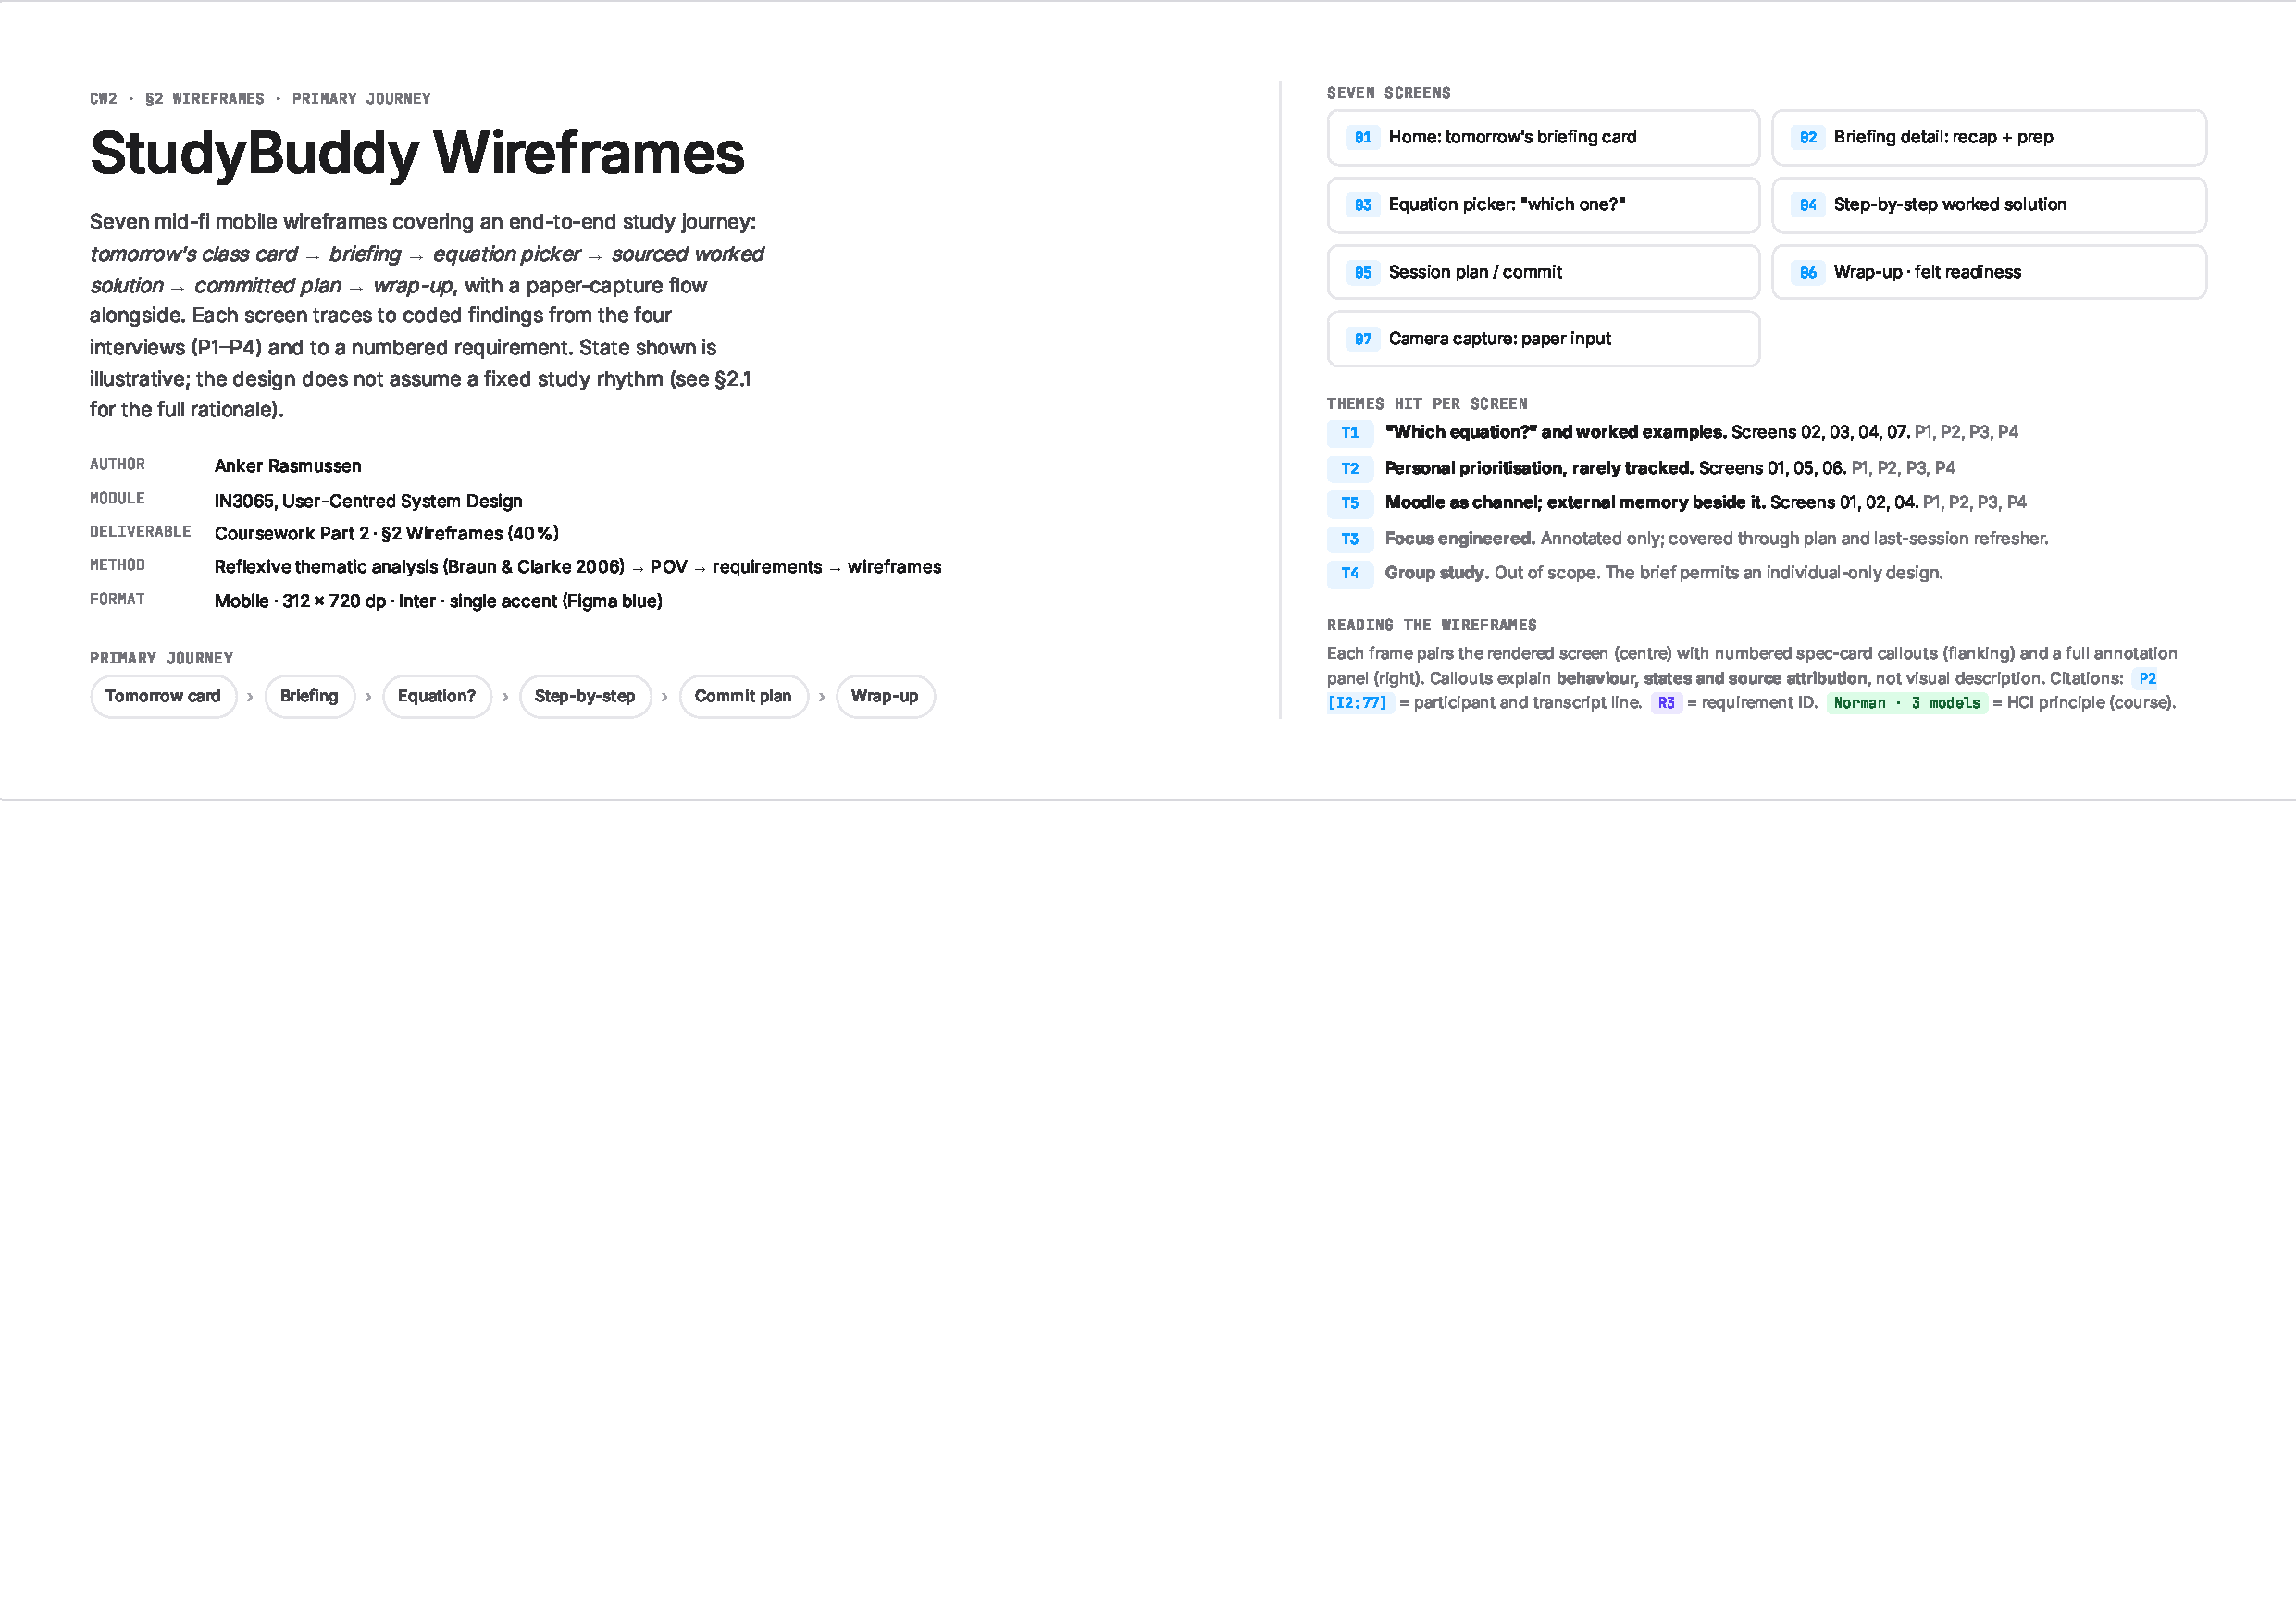
\includepdf[pages=-,pagecommand={\thispagestyle{fancy}}]{figures/wireframes.pdf}

% Placeholder per-wireframe stubs (replace with actual exports):
\subsubsection*{Wireframe 1: [screen name]}
% \includegraphics[width=\linewidth]{figures/wf-1.pdf}

\newpage
\subsubsection*{Wireframe 2: [screen name]}
% \includegraphics[width=\linewidth]{figures/wf-2.pdf}

\newpage
\subsubsection*{Wireframe 3: [screen name]}
% \includegraphics[width=\linewidth]{figures/wf-3.pdf}

\newpage
\subsubsection*{Wireframe 4: [screen name]}
% \includegraphics[width=\linewidth]{figures/wf-4.pdf}

\newpage
\subsubsection*{Wireframe 5: [screen name]}
% \includegraphics[width=\linewidth]{figures/wf-5.pdf}

\newpage
\subsubsection*{Wireframe 6: [screen name]}
% \includegraphics[width=\linewidth]{figures/wf-6.pdf}

% ============================================================
% SECTION 3: EVALUATION
% ============================================================
\newpage
\section{Usability Testing Plan}\label{sec:usability}
\wclimit{450}
% TODO: Evaluation aim; participants (who & how many); environment setup
% (City Interaction Lab), equipment, materials; what data is captured & how.
% 3 task scenarios with EXACT wording, what you hope to learn, and
% observable success criteria. Procedure with order + timing.

\subsubsection*{Evaluation Aim}
\subsubsection*{Participants}
\subsubsection*{Environment \& Equipment}
\subsubsection*{Data Captured}
\subsubsection*{Task Scenarios}
% Task 1 -- exact wording:
%   Learning goal:
%   Success criteria:
% Task 2 -- exact wording:
%   Learning goal:
%   Success criteria:
% Task 3 -- exact wording:
%   Learning goal:
%   Success criteria:
\subsubsection*{Procedure}

% ============================================================
% REFERENCES (brief: Harvard style, before appendices)
% ============================================================
\newpage
\printbibliography[heading=bibintoc]

% ============================================================
% APPENDICES (brief: each starts on new page, listed in ToC)
% ============================================================
\newpage
\appendix
\addcontentsline{toc}{section}{Appendices}

\section{Research Materials}\label{app:research-materials}
% Recruitment screener (Qualtrics) and any other research materials.
% 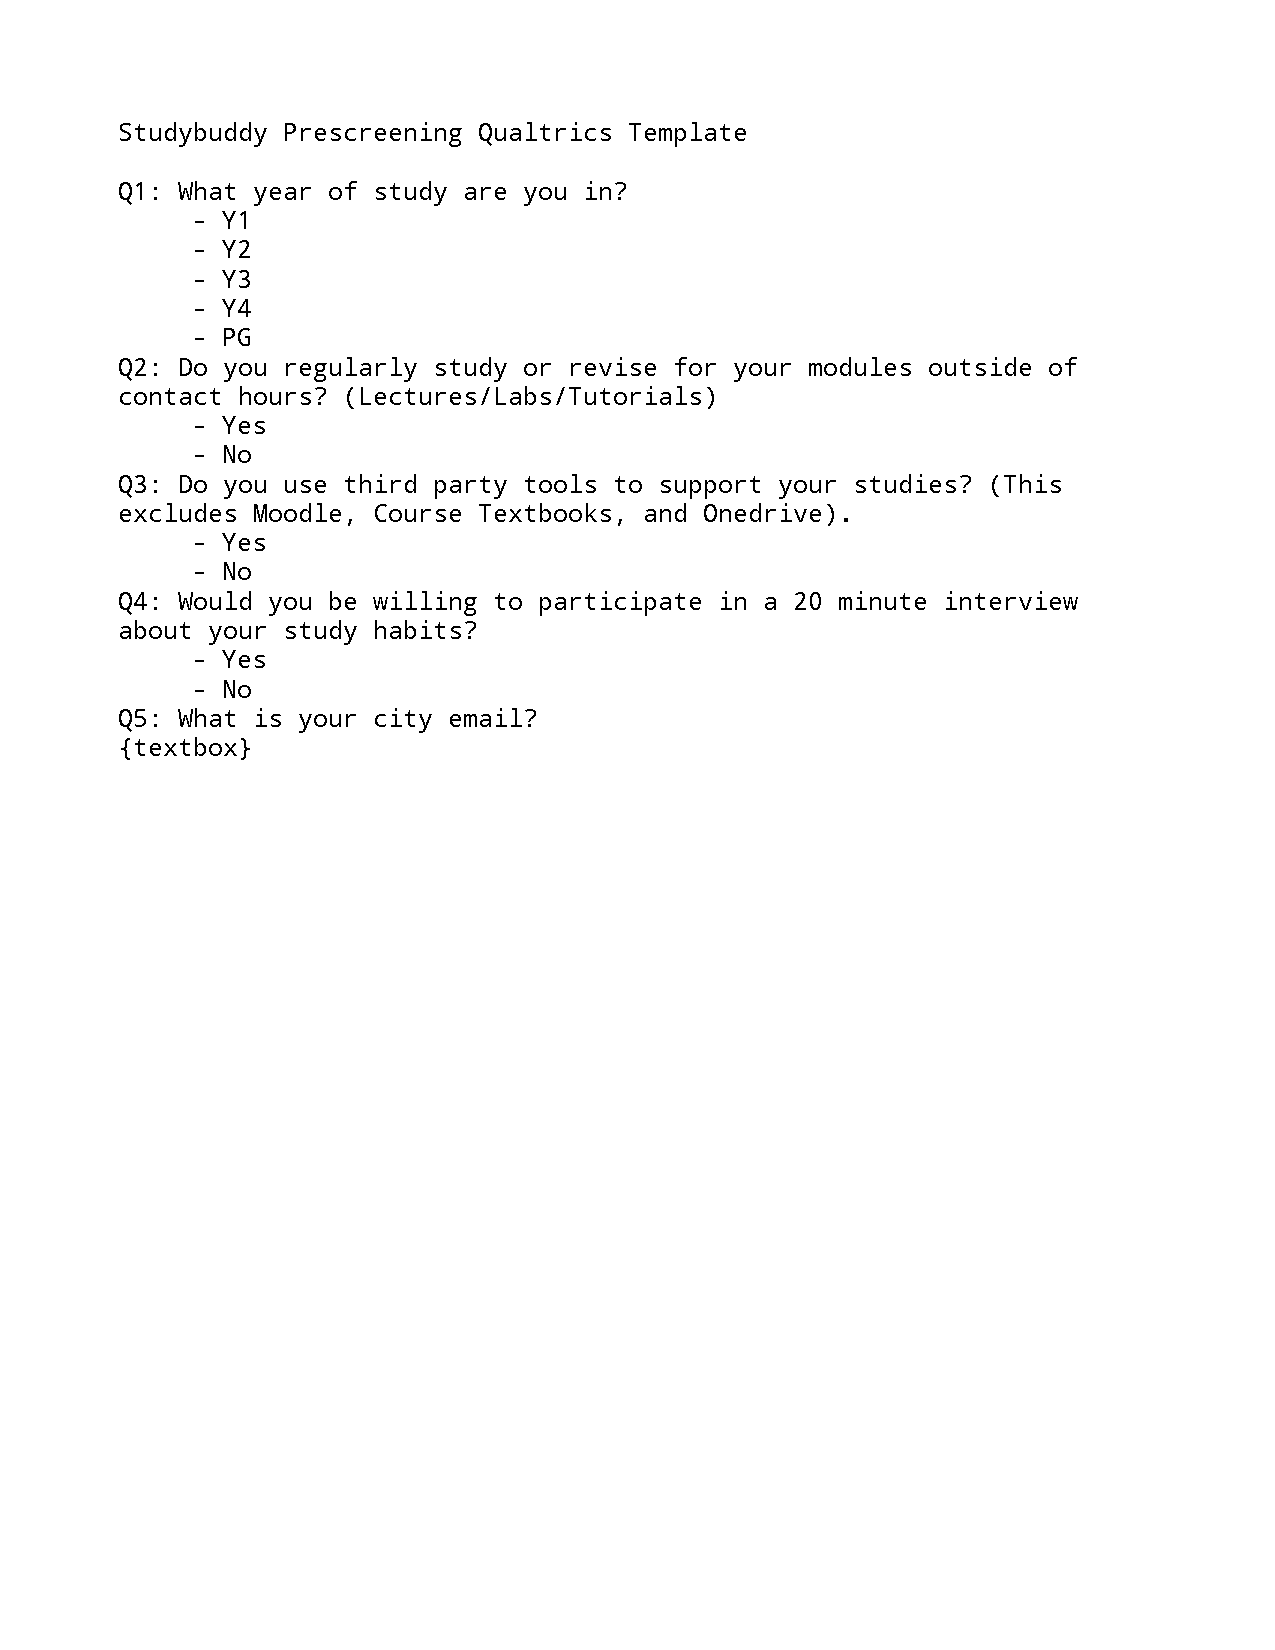
\includepdf[pages=-,pagecommand={\thispagestyle{fancy}}]{../Qualtrics.pdf}

\newpage
\section{Informed Consent Form Template (Final)}\label{app:consent}
% 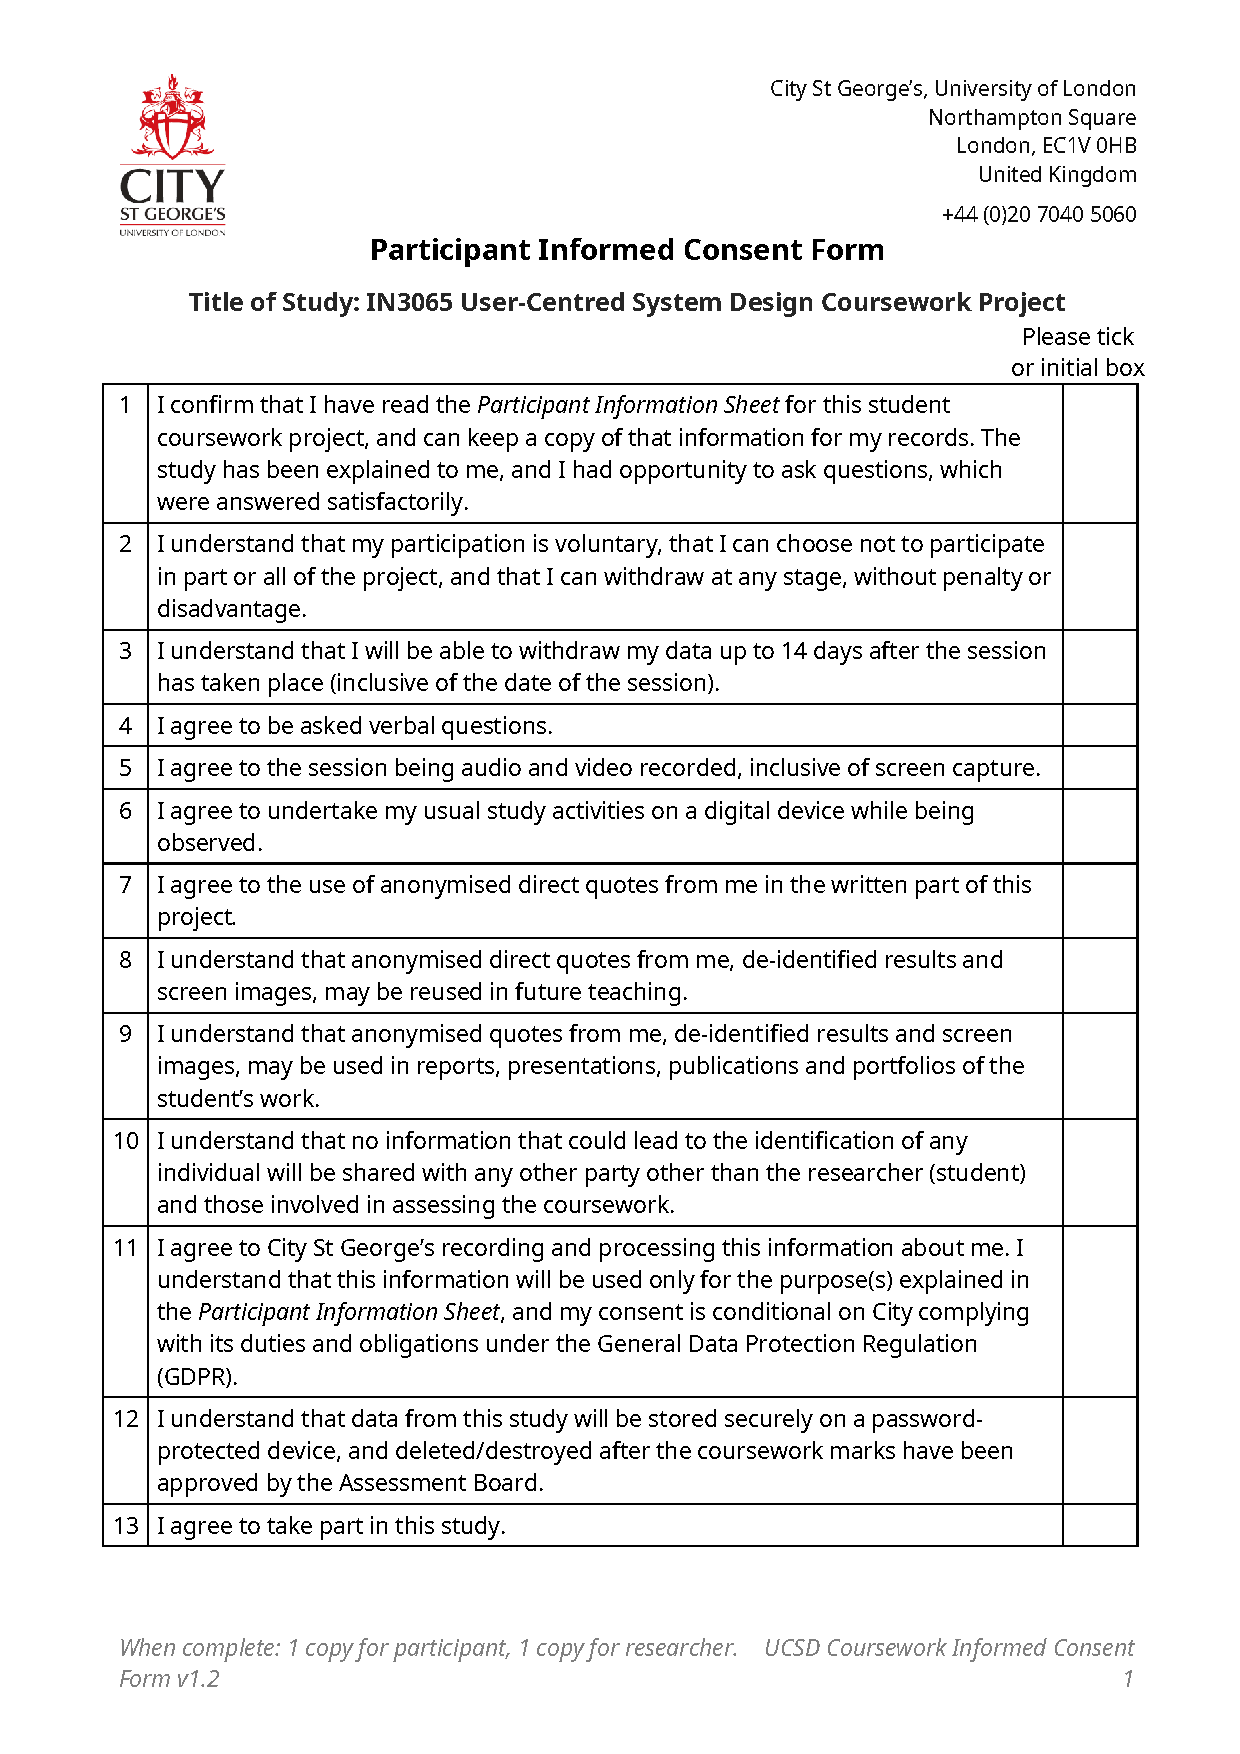
\includepdf[pages=-,pagecommand={\thispagestyle{fancy}}]{../UCSD-CW-Ethics-Informed Consent Form template-v1.2.pdf}

\newpage
\section{Participant Information Sheet (Final)}\label{app:pis}
% 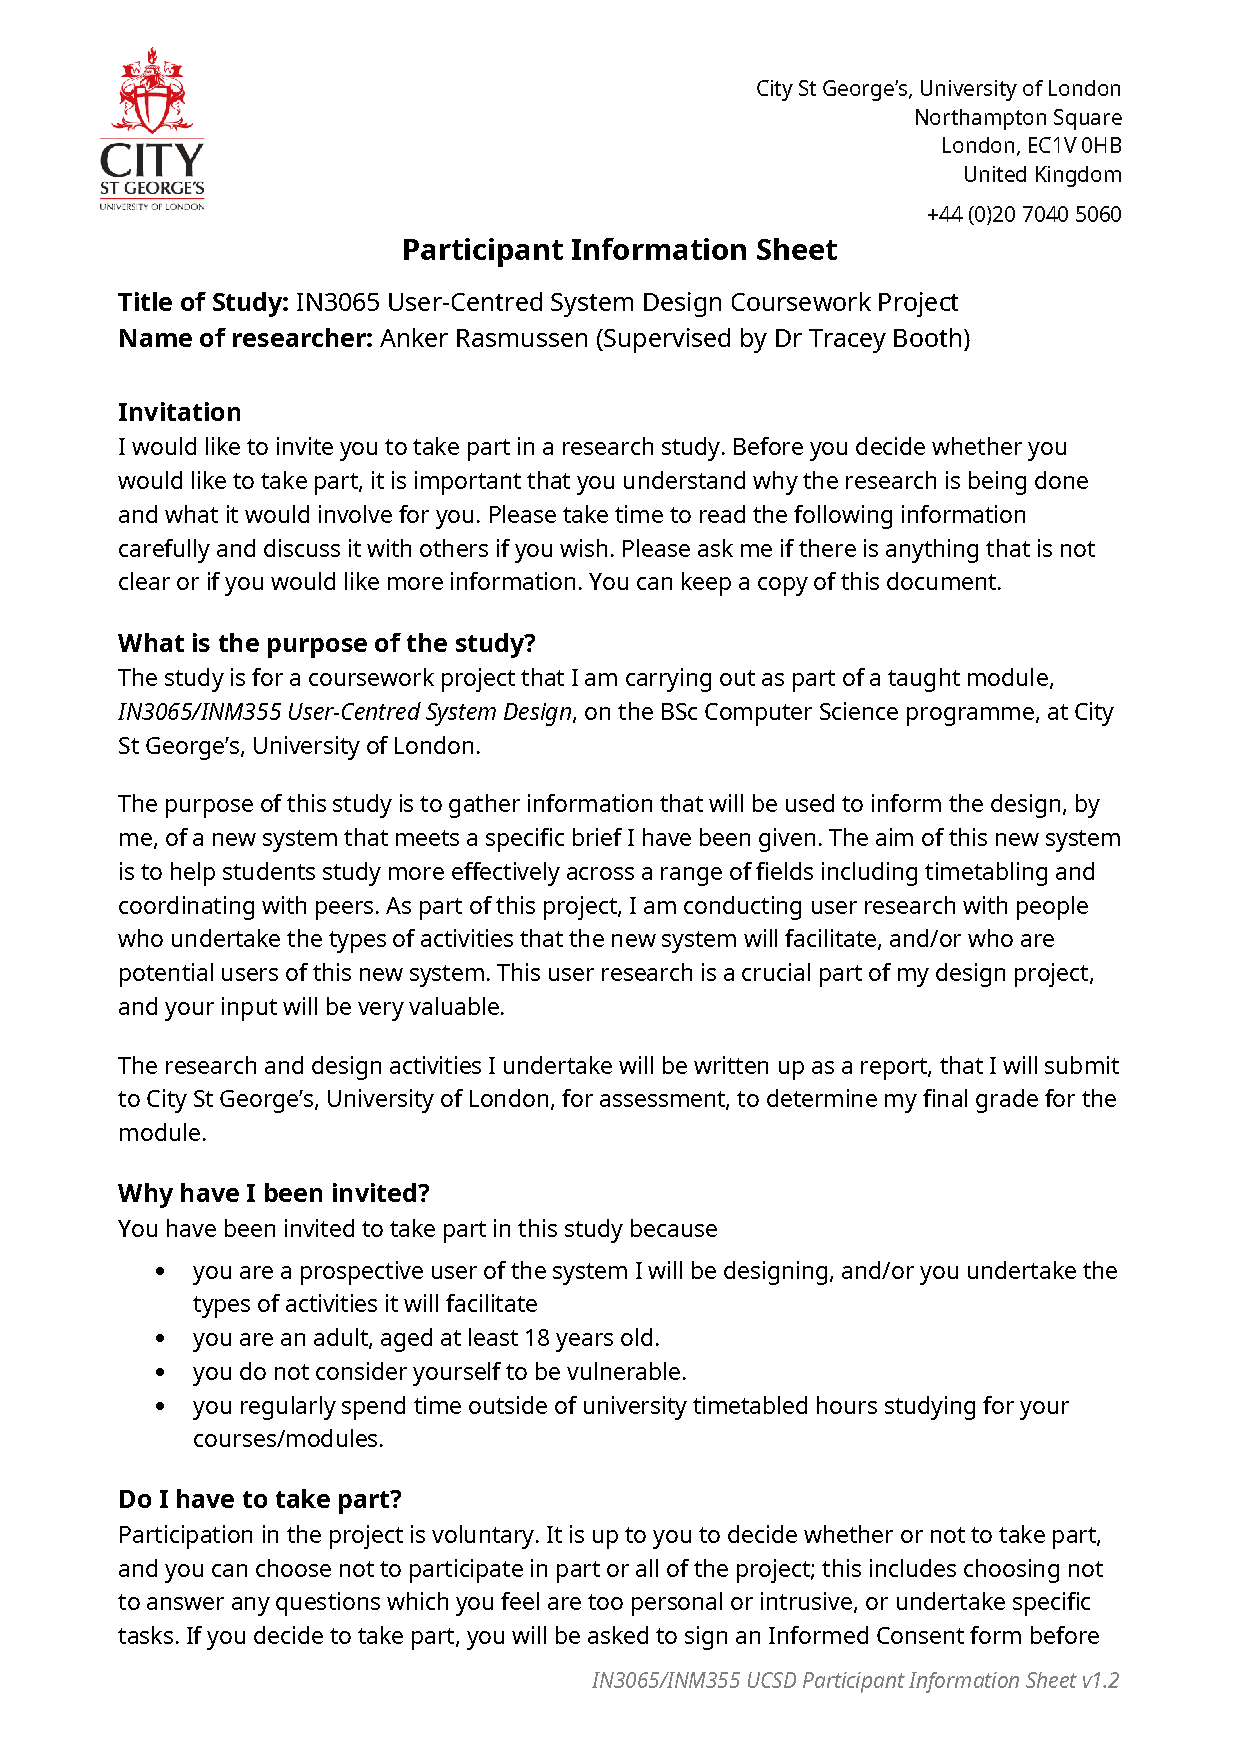
\includepdf[pages=-,pagecommand={\thispagestyle{fancy}}]{../UCSD-CW-Ethics-Participant Information Sheet template-v1.2.pdf}

\newpage
\section{Interview Guide / Script (Final)}\label{app:guide}
% Paste final, as-used version (may differ from CW1 draft).

\newpage
\section{Full List of Findings}\label{app:findings}
% Exhaustive list of findings/quotes from the interviews, P1--P4 tagged.

\newpage
\section{Interview Summaries}\label{app:summaries}
% Per-participant summary (P1--P4).

\newpage
\section{Evidence of Analysis}\label{app:analysis}
% Affinity diagram photos, coding tables, theme derivation, etc.

\newpage
\section{Observation / Walkthrough Notes}\label{app:observation}
% Notes + screenshots from the walkthrough portions of interviews.

% ============================================================
% GENAI USAGE LOG
% ============================================================
\newpage
\section{GenAI Usage Log}\label{app:genai}

The following table documents all use of Generative AI tools during the
preparation of CW2 materials, including prompts/inputs, outputs and uses.

\vspace{0.5em}
\noindent
\begin{longtable}{@{}p{1.8cm}p{2.8cm}p{4.5cm}p{4.5cm}@{}}
\toprule
\textbf{Date} & \textbf{Tool} & \textbf{Prompt/Input} & \textbf{Output \& Use} \\
\midrule
\endhead
2026-04-23
& Claude Opus 4.7 (Claude Code CLI)
& \texttt{start with a skeleton for pt2, and sections to logically
  work through.}
& Created \texttt{part-2/pt2.tex} as an empty skeleton mirroring the
  CW2 brief structure (cover page, User Research / Design /
  Usability Testing sections, References, Appendices and this
  GenAI log) and an empty \texttt{references.bib}. All section
  content left as TODO comments for the student to author. \\
\midrule
2026-04-24
& Claude Opus 4.7 (Claude Code CLI)
& \texttt{Write this to a md file for context for me.}
& Wrote \texttt{part-2/ROADMAP.md} as a personal working document
  (not a submission deliverable) capturing locked design direction,
  the planned wireframe journey, an analysis pipeline outline, a
  phase-by-phase checklist and a marking-weight table. No analytic
  content (findings, persona, wireframes) was generated. \\
\midrule
2026-04-25
& Claude Opus 4.7 (Claude Code CLI)
& \texttt{In Coursework I need to do some analysis of the
  interviews.} (with follow-up corrections redirecting to the CW2
  brief 1:1 and to thematic analysis as the single method.)
& Drafted \texttt{part-2/analysis.md} as a personal working
  analysis document (not submitted) applying Braun \& Clarke (2006)
  reflexive thematic analysis across the four cleaned transcripts:
  method block, participant table, per-interview summaries,
  line-level open codebooks, a code-cluster theme map, five named
  themes (T1--T5) with pull quotes, and a granular findings list
  F1--F49. All quotations cited by interview file and line; no
  content added to \texttt{pt2.tex} beyond this log entry. \\
\midrule
2026-04-26
& Claude Opus 4.7 (Claude Code CLI)
& \texttt{correct the onedrive folder url properly please.} +
  \texttt{can you take a look at my pt2?} + \texttt{clean all
  these up.}
& Cover-page OneDrive placeholder replaced with a clean
  \texttt{\textbackslash href} link. Cleanup pass on
  \texttt{pt2.tex} (no analytic content added): fixed a stray
  backtick in the URL; escaped a bare \texttt{\&} in \S1.1;
  repointed two undefined \texttt{\textbackslash ref} targets;
  added a \texttt{Research Materials} appendix as the resolution
  target for the Qualtrics-screener cite; deleted four duplicate
  empty subsection stubs in \S1.2; added a Braun \& Clarke 2006
  entry to \texttt{references.bib} and converted the inline
  citation to \texttt{\textbackslash textcite\{braun2006\}} so
  the bibliography is populated. \\
\midrule
2026-04-26
& Claude Opus 4.7 (Claude Code CLI)
& \texttt{tbf participant 3 did do a mini walkthrough but not as
  in depth as the others.} (student-supplied excerpt from
  \texttt{Interview3.md}.)
& Corrected the walkthrough count in \S1.1 from \emph{three of
  four} to \emph{all four}, and rewrote P3's blurb in \S1.2: P3
  gave a brief verbal scenario walkthrough only (no live setup
  or artefact). Mirror updates applied to \texttt{analysis.md}
  (method block, participant table, \S7 intro, and a new \S7.4
  with the verbal-walkthrough notes). The thematic analysis
  itself was carried out by the student. \\
\midrule
2026-04-26
& Claude Opus 4.7 (Claude Code CLI)
& \texttt{TBH I think the design goal would be better off focusing
  on t1 and t2.}
& Repivoted the \S1.2 Design Goal paragraph from T1+T4
  (worked-example gap + brittle pre-exam group study) to T1+T2
  (worked-example gap + personal, short-horizon prioritisation
  pattern); T5 retained as the coexistence constraint. Updated the
  Key Requirements list to drop the T4 peer-sessions bullet and
  add a T2 bullet requiring the system to adapt to the student's
  own prioritisation rule. Theme selection was the student's call. \\
\midrule
2026-04-26
& Claude Opus 4.7 (Claude Code CLI)
& \texttt{which template for figjam?} $\to$ \texttt{can you do it
  for me?}
& Generated \texttt{part-2/figjam-stickies.md}: a copy-paste source
  for building the Phase~3 affinity diagram in FigJam. Lifts the
  cluster contents from \texttt{analysis.md}~\S4 and reformats each
  cluster's codes as one-sticky-per-line blocks under labelled
  column headers (T1--T5 plus a ``Did not cluster'' group), with
  FigJam usage instructions at the top. No analytic content was
  generated; the clustering itself was the student's Phase~3 work.
  The exported PDF will be \texttt{\textbackslash includepdf}'d
  into Appendix~F. \\
\midrule
2026-04-27
& Claude Opus 4.7 (Claude Code CLI)
& \texttt{Is the affinity mapping from the 4 interviews accurate?
  Doublecheck (and take a look at figjam.pdf).} $\to$
  \texttt{quickly fix the figjam-stickies.md}
& Cross-checked every sticky in
  \texttt{part-2/figjam-stickies.md} against
  \texttt{Interview1--4.md} and against the rendered
  \texttt{figjam.pdf}. Reported back the (mostly accurate)
  attribution, plus three concrete bugs: a duplicated sticky
  (\emph{peer-asking only at exam season (P1)}) appearing in
  both T1 and T4, a typo (\emph{personal coding} $\to$
  \emph{personal colour-coding}) and 5~T1 stickies present in
  the .md but missing from the rendered board. Applied the
  duplicate-removal and typo fix to
  \texttt{figjam-stickies.md}; the figjam canvas itself
  was not modified. \\
\bottomrule
\end{longtable}

\end{document}
